\documentclass[10pt,a4paper, margin=1in]{article}
\usepackage{fullpage}
\usepackage{subcaption}
\usepackage{amsfonts, amsmath, pifont}
\usepackage{amsthm}
\usepackage{graphicx}
\usepackage{float}
\usepackage{wrapfig}
\usepackage{tkz-euclide}
\usepackage{tikz}
\usepackage{minted}
\usepackage{pgfplots}
\pgfplotsset{compat=1.13}

\usepackage{geometry}
 \geometry{
 a4paper,
 total={210mm,297mm},
 left=10mm,
 right=10mm,
 top=20mm,
 bottom=20mm,
 }

 \author{
  Geçit, Emre\\
  \texttt{e2521581@ceng.metu.edu.tr}
  \and
  Yancı, Baran\\
  \texttt{e2449015@ceng.metu.edu.tr}
}

\title{CENG 384 - Signals and Systems for Computer Engineers \\
Spring 2023 \\
Homework 1}
\begin{document}
\maketitle



\noindent\rule{19cm}{1.2pt}

\begin{enumerate}

\item %write the solution of q1
    \begin{enumerate}
    % Write your solutions in the following items.
    \item \begin{align*}
            &z = x + yj \implies \bar{z} = x - yj \\
            &2z + 5 = j - \bar{z} \\
            &2(x + yj) + 5 = j - (x - yj) \\
            &2x + 5 + 2yj = (1 + y)j - x \\
            &y = 1, x = \frac{-5}{3} \\
            &z = \frac{-5}{3} + j\\
            &|z|^2 = \frac{25}{9} + 1 = \frac{34}{9}
    \end{align*}

    % \includegraphics*[width=0.5\textwidth]{q1a.png}

    \begin{center}
        \begin{tikzpicture}

            \pgfplotsset{
                scale only axis,
            }
        
            \begin{axis}[
            xlabel=$real$,
            ylabel=$imaginary$,
            grid = both,
            xmin=-2, xmax=-1,
            ]
            \addplot[only marks, mark=*]
            coordinates{
                (-1.66, 1)
            }; \label{z}
        
                \addlegendimage{/pgfplots/refstyle=plot_one}
            \addlegendentry{z}
            \end{axis}
        
        \end{tikzpicture}
    \end{center}
      
        
    \item \begin{align*}
        & z = re^{j\theta} \implies z^5 = r^5e^{j5\theta} \\
        & 32j = 32e^{j\pi/2} \\
        & 32e^{j\pi/2} = r^5e^{j5\theta} \implies r = 2, \theta = \pi/10 \\
        & z = 2e^{j\pi/10}
    \end{align*}
    \item \begin{align*}
        z & = \frac{(1 + j) (\frac{1}{2} + \frac{\sqrt{3}}{2} j)}{j - 1} \\
        & = \frac{(j + 1) (1 + j) (\frac{1}{2} + \frac{\sqrt{3}}{2} j)}{(j + 1) (j - 1)} \\
        & = \frac{{(j + 1)}^2 (\frac{1}{2} + \frac{\sqrt{3}}{2} j)}{-2} \\
        & = \frac{(j^2 + 2j + 1) (\frac{1}{2} + \frac{\sqrt{3}}{2} j)}{-2} \\
        & = \frac{(-1 + 2j + 1) (\frac{1}{2} + \frac{\sqrt{3}}{2} j)}{-2} \\
        & = \frac{2j (\frac{1}{2} + \frac{\sqrt{3}}{2} j)}{-2} \\
        & = -j (\frac{1}{2} + \frac{\sqrt{3}}{2} j) \\
        & = - \frac{j}{2} + \frac{\sqrt{3}}{2} \\
        z & = r \cos\theta + r \sin\theta j \\
        - \frac{j}{2} + \frac{\sqrt{3}}{2} & = r \cos\theta + r \sin\theta j \\
        r\cos\theta & = \frac{\sqrt{3}}{2} \\
        r\sin\theta & = - \frac{1}{2} \\
        r & = 1 \\
        \theta & = \frac{-\pi}{6} \\
    \end{align*}
    \item \begin{align*}
        z & = je^{-j\pi/2} \\
        & = e^{j\pi/2}e^{-j\pi/2} \\
        & = e^0 = 1
    \end{align*}
    \end{enumerate}

\newpage % start a new page so that the layout of the graph is not messed up.
\item %write the solution of q2
    The graph of the function is given below.
    \begin{center}
        \includegraphics*[width=0.5\textwidth]{assets/graphs/q2.png}
    \end{center}

\item %write the solution of q3
    \begin{enumerate}
    % Write your solutions in the following items.
    \item
        The graph of the function $x[-n] + x[2n - 1]$ is given below.
        \begin{center}
            \includegraphics*[width=0.5\textwidth]{assets/graphs/q3a.png}
        \end{center}
    \item \begin{align*}
        x[n] &=  -\delta[n-1] + 2\delta[n-2] + -4\delta[n-4] + 3\delta[n-7] \\
        x[-n] &= -\delta[-n-1] + 2\delta[-n-2] + -4\delta[-n-4] + 3\delta[-n-7] \\
        &= -\delta[n+1] + 2\delta[n+2] + -4\delta[n+4] + 3\delta[n+7] \\
        x[2n-1] &= -\delta[2n-2] + 2\delta[2n-3] + -4\delta[2n-5] + 3\delta[2n-8] \\
        &= -\delta[n-1] + 3\delta[n-4] \\
        x[-n] + x[2n-1] &= -\delta[n+1] + 2\delta[n+2] + -4\delta[n+4] + 3\delta[n+7] + -\delta[n-1] + 3\delta[n-4] \\
    \end{align*}
    
    
    \end{enumerate}

\item %write the solution of q4
    \begin{enumerate}
    \item \begin{align*}
        period(5\sin(3t - \frac{\pi}{4})) & = period(\sin(3t)) && \text{Scaling the amplitude does not affect the period, neither does shifting.} \\
        & = period(\sin(t)) / 3 && \text{Time scaling inversely affects the period.} \\
        & = \frac{2\pi}{3} && \text{Period of sin is } 2\pi. \\
    \end{align*}    
    \item $cos[\frac{13\pi}{10}n]$ is periodic with period $\frac{2\pi*10}{13\pi} = \frac{20}{13}$
    
    $sin[\frac{7\pi}{10}n]$ is periodic with period $\frac{2\pi*10}{7\pi} = \frac{20}{7}$

    Least common multiple of $\frac{20}{13}$ and $\frac{20}{7}$ is $20$, which is also an integer, so it satisfies the discrete-time periodicity condition.

	\item In order $\frac{1}{2}\cos[7n - 5]$ to be periodic, its continuous-time counterpart must have a rational period.
    However, the signal $\frac{1}{2}\cos(7n - 5)$ has a fundamental period of $2\pi/7$.

    There is no integer $t_0$ such that,
    \begin{align*}
        \frac{1}{2}\cos[7n - 5] & = \frac{1}{2}\cos[7(n + t_0) - 5] \\
    \end{align*}
    \end{enumerate}

\item %write the solution of q5
    \begin{enumerate}
    \item $x(t) = u[t-1] - 3u[t-3] + u[t-4]$
    \item $\frac{dx(t)}{dt} = \delta(t-1) -3\delta(t-3) +\delta(t-4)$
        The graph of $\frac{dx(t)}{dt}$ is given below.
        \begin{center}
            \includegraphics*[width=0.5\textwidth]{assets/graphs/q5b.png}
        \end{center}
    \end{enumerate}    
    
\item %write the solution of q6
    \begin{enumerate}
    % Write your solutions in the following items.
    \item %write the solution of q6a
        \begin{align*}
            y(x) & = tx(2x + 3) \\
        \end{align*}
        \textit{Memory: } The system has memory, as the output depends on the future values of the input.
        For example, for $t = 3$, the output value depends on the future value of the input, $y(3) = 3x(9)$.\\
        \textit{Stability: } The system is \textbf{not} stable, as there is no finite number $b'$ such that $|y(t)| \leq b'$ for all $t$.\\
        \textit{Causality: } The system is \textbf{not} causal, as the output depends on the future values of the input.\\
        \textit{Linearity: } The system is linear, because the superposition principle holds.\\
        \begin{align*}
            x_1 \implies y_1(t) & = tx_1(2t + 3) \\
            x_2 \implies y_2(t) & = tx_2(2t + 3) \\
            x_3 & = a_1x_1 + a_2x_2 & assumption\\
            y_3 & = t(a_1x_1 + a_2x_2) = a_1y_1 + a_2y_2 \\
        \end{align*}
        \textit{Invertibility: } The system is invertible for $t \neq 3$.
        \begin{align*}
            y(t) & = tx(2t + 3) \\
            \frac{1}{t}y(t) & = x(2t + 3) \\
            \frac{2}{t - 3}y\left(\frac{t - 3}{2}\right) & = x(t) \\
        \end{align*}
        \textit{Time invariance: } The system is \textbf{not} time invariant.
        \begin{align*}
            y(t) & = tx(2t + 3) \\
            y(t - t_0) = (t-t_0)x(2(t - t_0) + 3) & \neq tx(2(t - t_0) + 3) \\
        \end{align*}
    \item %write the solution of q6b
        \begin{align*}
            y[n] & = \sum_{k = 1}^{\infty} x[n - k] \\
        \end{align*}
        \textit{Memory: } The system has memory, as the output depends on the past values of the input.
        For example, for $n = 6$, the output value depends on the past values of the input,
        $y[6] = x[5] + x[4] + x[3] + \cdots$.\\
        \textit{Stability: } The system is \textbf{not} stable, as there is no finite number $b'$ such that $|y(t)| \leq b'$ for all $t$.
        For example, if we take $x(n)$ as the unit step function, the signal $\sum_{k = 1}^{\infty} u[n - k]$ is unbounded for $n \implies \infty$.\\
        \textit{Causality: } The system is causal, as the output depends on the past values of the input.\\
        \textit{Linearity: } The system is linear, because the superposition principle holds.\\
        \begin{align*}
            x_1 \implies y_1(n) & = \sum_{k = 1}^{\infty} x_1[n - k] \\
            x_2 \implies y_2(n) & = \sum_{k = 1}^{\infty} x_2[n - k] \\
            a_1y_1 + a_2y_2 & = \sum_{k = 1}^{\infty} (a_1x_1[n - k] + a_2x_2[n - k])\\
            \sum_{k = 1}^{\infty} x_3[n - k] & = a_1\sum_{k = 1}^{\infty} x_1[n - k] + a_2\sum_{k = 1}^{\infty} x_2[n - k] \\ 
        \end{align*}
        \textit{Invertibility: } The system is invertible, the fact that the system has the invertibility property can be seen
        by taking the difference of two consequent values of $y[n]$.\\
        \begin{align*}
            y[n + 1] - y[n] & = \sum_{k = 1}^{\infty} x[n + 1 - k] - \sum_{k = 1}^{\infty} x[n - k]\\
            y[n + 1] - y[n] & = x[n]\\
        \end{align*}
        \textit{Time invariance: } The system is time invariant, because a delay in the input signal $x[n]$ by $x$, causes a
        corresponding delay for the output signal $y[n]$ by $x$ as well.\\
        \begin{align*}
            y[n] & = \sum_{k = 1}^{\infty} x[n - k] \\
            y[n- n_0] & = \sum_{k = 1}^{\infty} x[(n - n_0) - k]\\
        \end{align*}
        \end{enumerate}
    
\item %write the solution of q7
    \begin{enumerate}
    \item \hfill\begin{minted}{python}
def decompose(signal_name):
    """Read the CSV file with the signal name, decompose the signal into even and odd components,
    and save the results as PNG files."""

    with open(signal_name + ".csv", "r", encoding="ascii") as file:
        data = [float(item) for item in file.read().split(",")]
    start = int(data[0])
    signal = data[1:]
    end = start + len(signal) - 1

    pyplot.title("Original Signal")
    pyplot.plot(range(start, end + 1), signal)
    pyplot.savefig(IMAGES_PATH + signal_name + "_original.png")
    pyplot.clf()

    if abs(start) > end:
        signal = signal + [0] * (abs(start) - end)
        end = -start
    else:
        signal = [0] * (end - abs(start)) + signal
        start = -end

    even = [(x + y) / 2 for x, y in zip(signal, signal[::-1])]
    odd = [(x - y) / 2 for x, y in zip(signal, signal[::-1])]

    pyplot.title("Even Component")
    pyplot.plot(range(start, end + 1), even)
    pyplot.savefig(IMAGES_PATH + signal_name + "_even.png")
    pyplot.clf()

    pyplot.title("Odd Component")
    pyplot.plot(range(start, end + 1), odd)
    pyplot.savefig(IMAGES_PATH + signal_name + "_odd.png")
    pyplot.clf()
\end{minted}

\begin{figure}[H]
    \centering
    \begin{subfigure}[t]{0.3\linewidth}
    \centering
        \caption{Original Signal}
        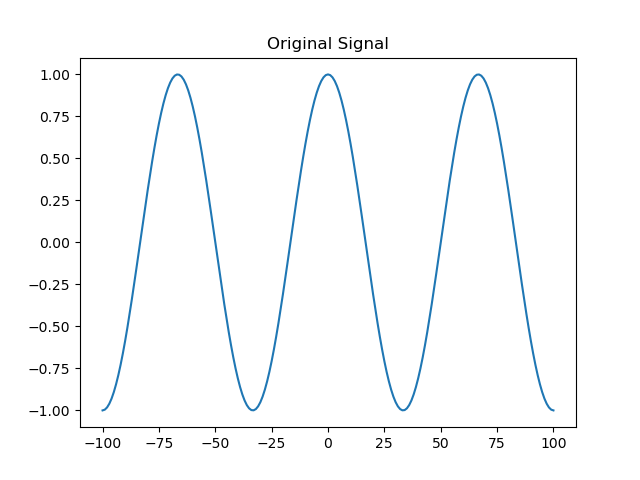
\includegraphics[width=1\linewidth]{assets/q7a/sine_part_a_original.png}
    \end{subfigure}
    \begin{subfigure}[t]{0.3\linewidth}
    \centering
        \caption{Even Component}
        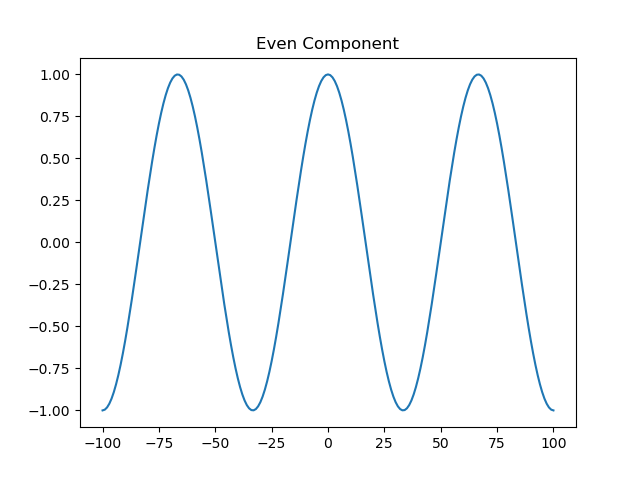
\includegraphics[width=1\linewidth]{assets/q7a/sine_part_a_even.png}
    \end{subfigure}
    \begin{subfigure}[t]{0.3\linewidth}
    \centering
        \caption{Odd Component}
        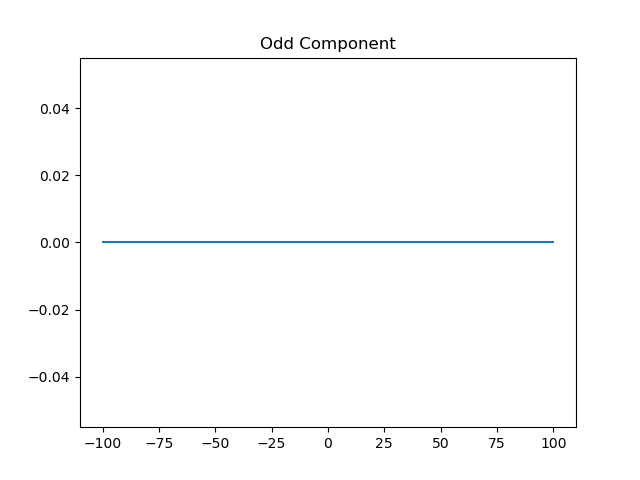
\includegraphics[width=1\linewidth]{assets/q7a/sine_part_a_odd.png}
    \end{subfigure}
    \caption{Sinusoidal Signal Decomposition}
\end{figure}

\begin{figure}[h]
    \centering
    \begin{subfigure}[t]{0.3\linewidth}
        \centering
        \caption{Original Signal}
        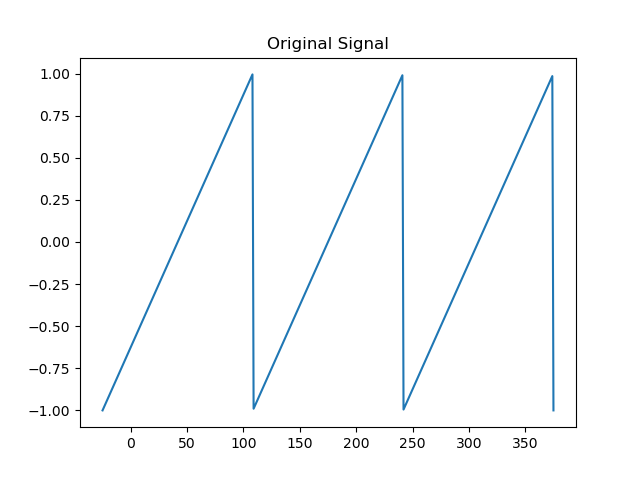
\includegraphics[width=1\linewidth]{assets/q7a/shifted_sawtooth_part_a_original.png}
    \end{subfigure}
    \begin{subfigure}[t]{0.3\linewidth}
        \centering
        \caption{Even Component}
        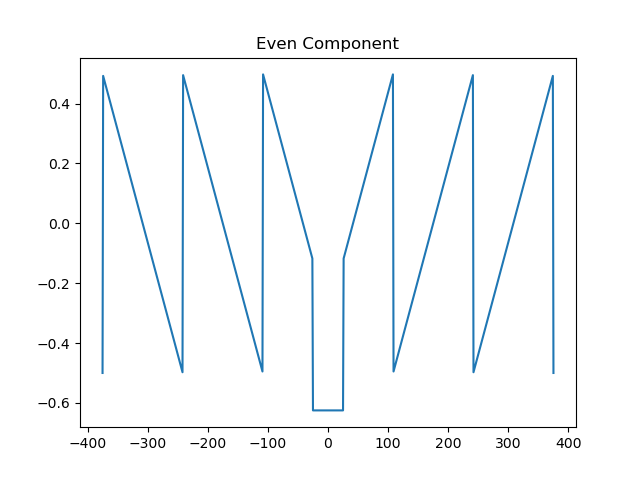
\includegraphics[width=1\linewidth]{assets/q7a/shifted_sawtooth_part_a_even.png}
    \end{subfigure}
    \begin{subfigure}[t]{0.3\linewidth}
        \centering
        \caption{Odd Component}
        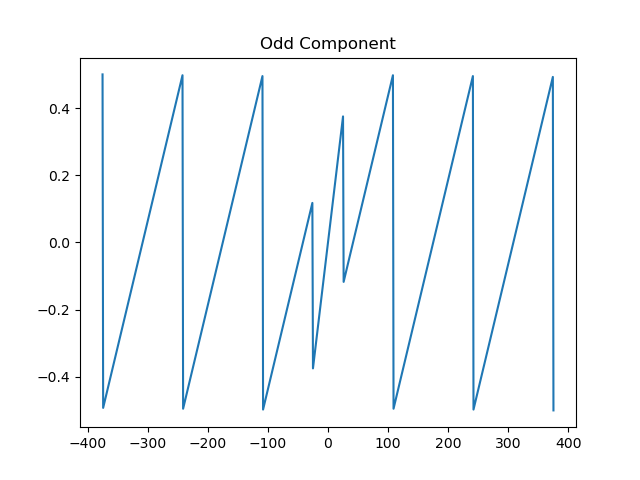
\includegraphics[width=1\linewidth]{assets/q7a/shifted_sawtooth_part_a_odd.png}
    \end{subfigure}
    \caption{Shifted Sawtooth Signal Decomposition}
\end{figure}

\begin{figure}[H]
    \centering
    \begin{subfigure}[t]{0.3\linewidth}
        \centering
        \caption{Original Signal}
        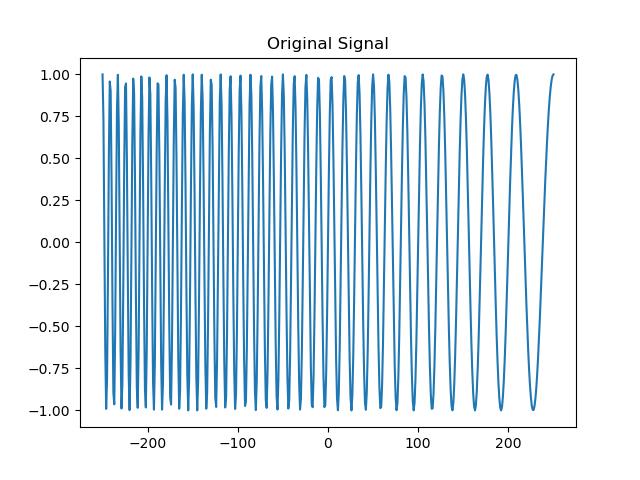
\includegraphics[width=1\linewidth]{assets/q7a/chirp_part_a_original.png}
    \end{subfigure}
    \begin{subfigure}[t]{0.3\linewidth}
        \centering
        \caption{Even Component}
        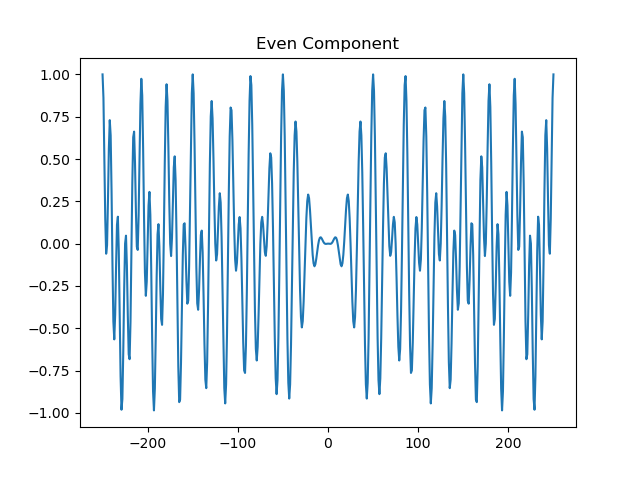
\includegraphics[width=1\linewidth]{assets/q7a/chirp_part_a_even.png}
    \end{subfigure}
    \begin{subfigure}[t]{0.3\linewidth}
        \centering
        \caption{Odd Component}
        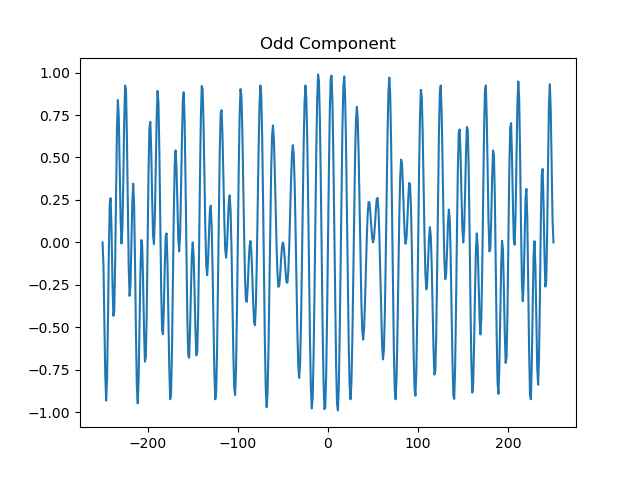
\includegraphics[width=1\linewidth]{assets/q7a/chirp_part_a_odd.png}
    \end{subfigure}
    \caption{Chirp Signal Decomposition}
\end{figure}


    

    \item \hfill \begin{minted}{python}
def shift_n_scale(signal_name):
    """
    Read the CSV file with the signal name, shift and scale the signal,
        and save the results as PNG files.

    This functions reads a signal x[n], and produces x[a*n + b] for a and b.
    """

    with open(signal_name + ".csv", "r", encoding="ascii") as file:
        data = [float(item) for item in file.read().split(",")]
    start = int(data[0])
    a = int(data[1])
    b = int(data[2])
    signal = data[3:]
    end = start + len(signal) - 1

    new_start = (start - b) // a
    new_end = (end - b) // a
    pyplot.xlim(new_start, new_end)

    pyplot.plot(range(start, end + 1), signal,linewidth=1)

    if new_start > new_end:
        domain = range(new_start, new_end, -1)
    else:
        domain = range(new_start, new_end + 1)
    pyplot.plot(
        domain,
        [signal[a*i+b-start] for i in domain],
        linewidth=1,
    )
    pyplot.legend(
        ["x[n]",
        "x[" + (str(a) if a != 1 else "") + "n " + ("+" if b >= 0 else "") + str(b) + "]"],
        loc="lower right",
        fontsize=8,
    )
    pyplot.savefig(IMAGES_PATH + signal_name)
    pyplot.clf()
    \end{minted}
    \end{enumerate}    

\end{enumerate}

\begin{figure}[H]
    \centering
    \begin{subfigure}[t]{0.3\linewidth}
        \centering
        \caption{Sinusoidal Signal}
        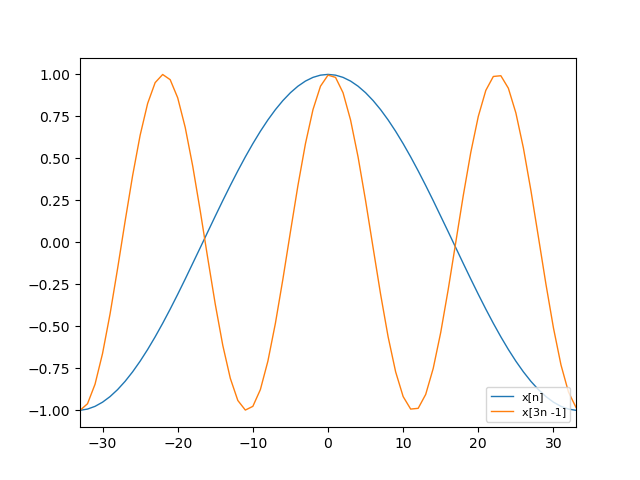
\includegraphics[width=1\linewidth]{assets/q7b/sine_part_b.png}
    \end{subfigure}
    \begin{subfigure}[t]{0.3\linewidth}
        \centering
        \caption{Shifted Sawtooth Signal}
        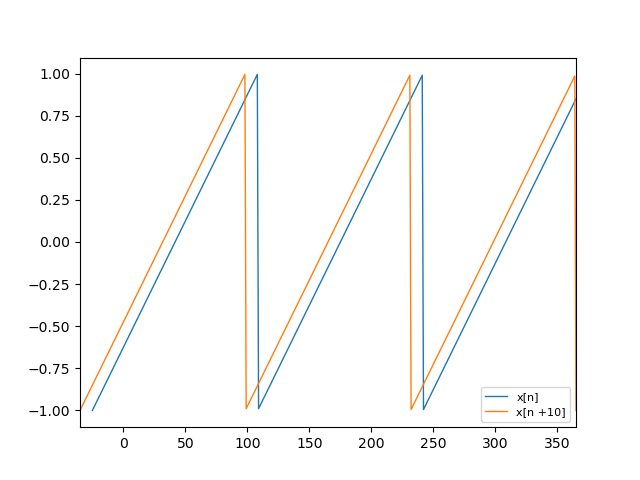
\includegraphics[width=1\linewidth]{assets/q7b/shifted_sawtooth_part_b.png}
    \end{subfigure}
    \begin{subfigure}[t]{0.3\linewidth}
        \centering
        \caption{Chirp Signal}
        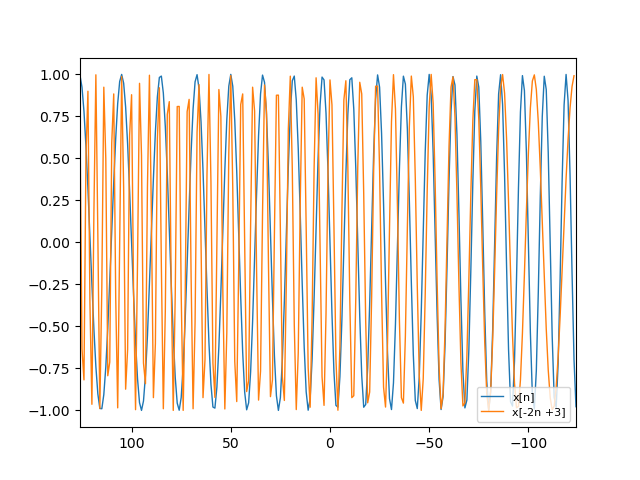
\includegraphics[width=1\linewidth]{assets/q7b/chirp_part_b.png}
    \end{subfigure}
    \caption{Shift and Scale}
\end{figure}

\end{document}

